%%%%%%%%%%%%%%%%%%%%%%%%%%%%%%%%%%%%%%%%%%%%%%%%%%%%
% LECTURE 17
%%%%%%%%%%%%%%%%%%%%%%%%%%%%%%%%%%%%%%%%%%%%%%%%%%%%
\section*{Internal Flow Analysis and Temperature Distributions}
\addcontentsline{toc}{section}{Internal Flow Analysis and Temperature Distributions}
%%%%%%%%%%%%%%%%%%%%%%%%%%%%%%%%%%%%%%%%%%%%%%%%%%%%
\subsection*{Energy Balance in Internal Flows}
\addcontentsline{toc}{subsection}{Energy Balance in Internal Flows}
%%%%%%%%%%%%%%%%%%%%%%%%%%%%%%%%%%%%%%%%%%%%%%%%%%%%
For internal flows, we perform an energy balance on a control volume between $x$ and $x+dx$:
%
\begin{figure}[H]
    \centering
    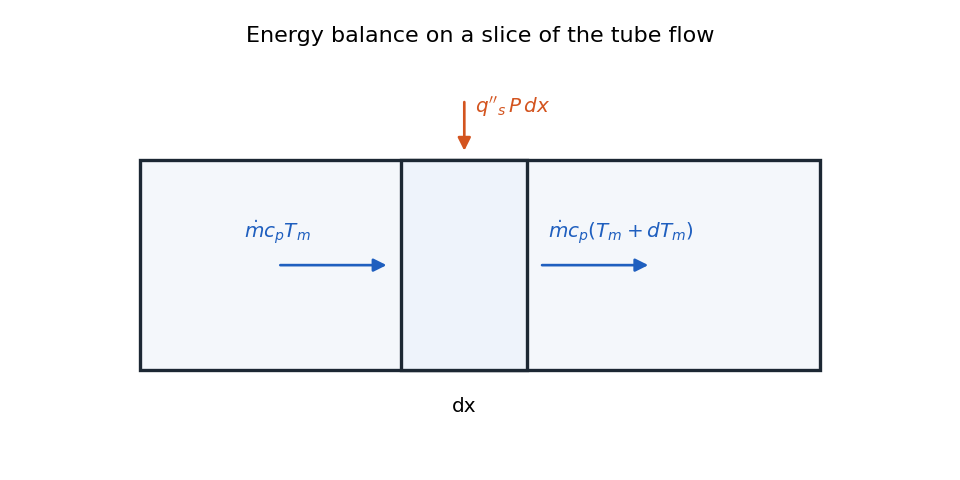
\includegraphics[width=0.65\linewidth]{pics/control_volume_pipe.png}
    \caption{Control volume for internal flow in a tube.}
\end{figure}
%
Energy in:
\begin{itemize}
    \item Advection: $\dot{m}c_pT_m$
    \item Heat through surface: $q''_sP\,dx$
\end{itemize}

Energy out:
\begin{itemize}
    \item Advection: $\dot{m}c_p(T_m + dT_m)$
\end{itemize}

For steady state, the balance yields:
\[
q''_sP\,dx = \dot{m}c_p\,dT_m
\]

Or:
\[
    \boxed{
        \frac{dT_m}{dx} = \frac{q''_sP}{\dot{m}c_p}
        }
\]

Using the definition of heat transfer coefficient:
\[
    q''_s = h(T_s - T_m)
\]

The energy balance becomes:
\[
    \boxed{
        \frac{dT_m}{dx} = \frac{hP}{\dot{m}c_p}(T_s - T_m)
        }
\]

\subsection*{Case 1: Constant Heat Flux}
\addcontentsline{toc}{subsection}{Case 1: Constant Heat Flux}

For constant heat flux ($q''_s = \text{constant}$), the mean temperature increases linearly:
\[
\frac{dT_m}{dx} = \frac{q''_sP}{\dot{m}c_p} = \text{constant}
\]

Therefore:
\[
T_m(x) = T_{m,i} + \frac{q''_sP}{\dot{m}c_p}x
\]

where $T_{m,i}$ is the inlet temperature.

The surface temperature can be determined from:
\begin{definition}
  \[
    T_s(x) = T_m(x) + \frac{q''_s}{h(x)}
    \]  
\end{definition}
%
In the fully developed region where $h$ is constant, the surface temperature also increases linearly with the same slope as the bulk temperature, maintaining a constant temperature difference:
\[
T_s(x) - T_m(x) = \frac{q''_s}{h} = \text{constant for } x > x_{fd,t}
\]
%
In the entrance region, the heat transfer coefficient is higher, resulting in a smaller temperature difference near the inlet. The surface temperature profile will have a non-linear portion in the entrance region before becoming linear in the fully developed region.

\subsection*{Case 2: Constant Surface Temperature}
\addcontentsline{toc}{subsection}{Case 2: Constant Surface Temperature}
%
For constant surface temperature ($T_s = \text{constant}$), the energy balance is:
%
\[
    \frac{dT_m}{dx} = \frac{\bar{h}P}{\dot{m}c_p}(T_s - T_m)
\]
%
Assuming $\bar{h}$ is constant (valid for the fully developed region), this can be integrated:
\begin{definition}
 \[
    \frac{T_s - T_m(x)}{T_s - T_{m,i}} = \exp \left(-\frac{\bar{h}\,P }{\dot{m} c_p}\,x \right)
\]   
\end{definition}
%
The mean temperature approaches the surface temperature exponentially, Figure \ref{fig:delta_T_vs_x_pipe}. It can be proven over a pipe of length $L$
\begin{definition}
    \[
        \frac{\Delta T_0}{\Delta T_i}=\frac{T_s-T_{m, 0}}{T_s-T_{m, i}}=\exp \left(-\frac{P L}{\dot{m} c_p} \bar{h}\right)
\]
\end{definition}
%
The total heat transfer rate is:
\begin{definition}   
    \[
        \begin{aligned}
            q &= \dot{m}c_p[T_m(x) - T_i] = \dot{m}c_p(T_s - T_i)(1 - e^{-\frac{\bar{h}P}{\dot{m}c_p}\,x})
            \\[0.5em]
            q &= \dot{m}c_p \Delta T = \rho c_p u_m A_c\Delta T
        \end{aligned}
    \]
\end{definition}

%
\begin{figure}[H]
    \centering
    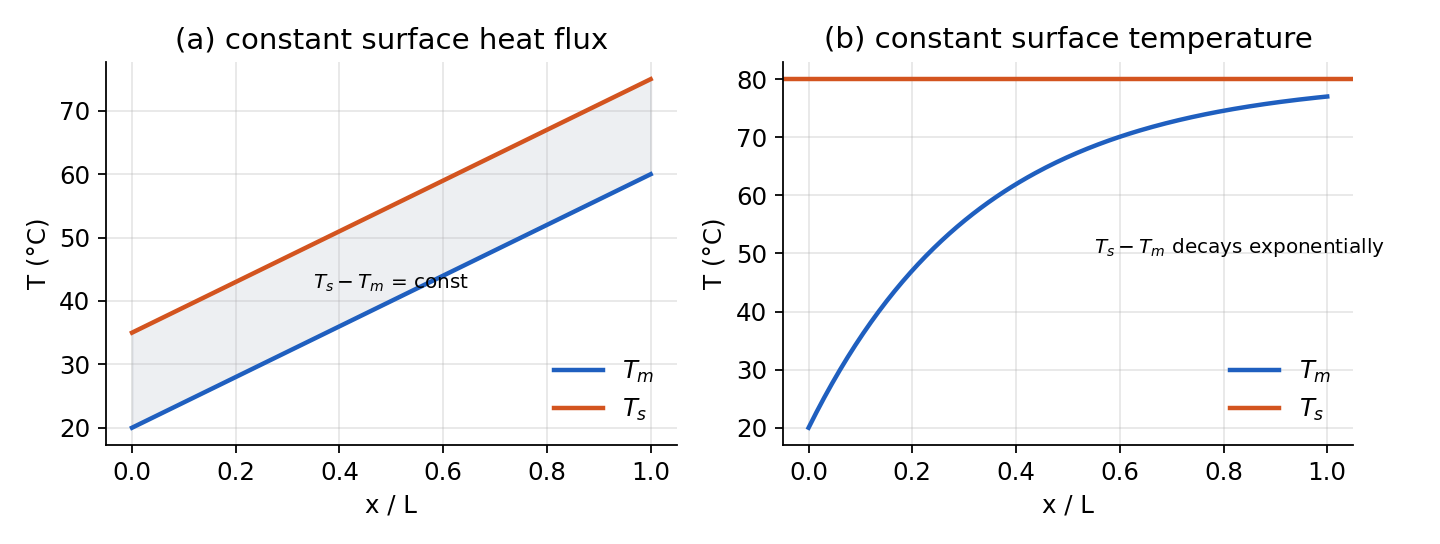
\includegraphics[width=0.85\linewidth]{pics/axial_temp_pipe.png}
    \caption{Axial temperature variations for heat transfer in a tube. (a) Constant surface heat flux. (b) Constant surface temperature.}
    \label{fig:delta_T_vs_x_pipe}
\end{figure}
%%%%%%%%%%%%%%%%%%%%%%%%%%%%%%%%%%%%%%%%%%%%%%%%%%%%%
\subsection*{Log Mean Temperature Difference (LMTD)}
\addcontentsline{toc}{subsection}{Log Mean Temperature Difference (LMTD)}
%%%%%%%%%%%%%%%%%%%%%%%%%%%%%%%%%%%%%%%%%%%%%%%%%%%%%

For heat exchanger applications, it's useful to define the log mean temperature difference:
\[
\Delta T_{lm} = \frac{\Delta T_i - \Delta T_o}{\ln(\Delta T_i/\Delta T_o)}
\]

where:
\begin{itemize}
    \item $\Delta T_i = T_s - T_i$ (inlet temperature difference)
    \item $\Delta T_o = T_s - T_o$ (outlet temperature difference)
\end{itemize}

This allows the total heat transfer to be expressed simply as:
\[
    \begin{aligned}
        q_{c a n \nu} &=\dot{m} c_{p}\, \Delta T_{l m} \cdot \ln \left(\Delta T_0 / \Delta T_i\right) \cdot(-1)
        \\[1em]
        & = \dot{m} c_p \cdot \Delta T_{l m} \cdot\left(-\frac{P L}{\dot{m} c_p} \bar{h}\right)(-1)
        \\[0.5em]
        & = \bar{h} \cdot PL\cdot \Delta_{lm}
        \\[0.5em]
        & = \bar{h}A_s \Delta T_{lm}
    \end{aligned}
\]
\begin{definition}
    \[
        q_{conv} = \bar{h}A_s \Delta T_{lm}
    \]
\end{definition}
%
The LMTD is useful for heat exchanger design because:
\begin{itemize}
    \item It represents an effective temperature difference for the entire heat exchanger
    \item It's convenient for experimental measurements (only need inlet and outlet temperatures)
    \item It simplifies heat exchanger calculations
\end{itemize}
%%%%%%%%%%%%%%%%%%%%%%%%%%%%%%%%%%%%%%%%%%%%%%%%%%%%%%%%%%%%%%
\subsubsection*{Internal heat flow summary}
\addcontentsline{toc}{subsubsection}{Internal heat flow summary}
%%%%%%%%%%%%%%%%%%%%%%%%%%%%%%%%%%%%%%%%%%%%%%%%%%%%%%%%%%%%%%

\begin{figure}[H]
    \centering
    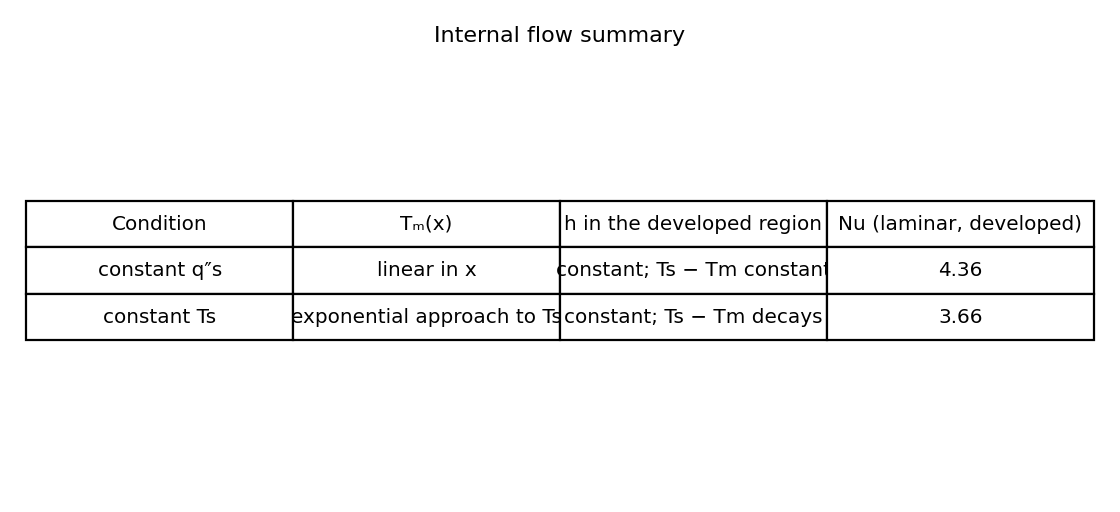
\includegraphics[width=0.95\linewidth]{pics/internal_heat_flow_summary.png}
    \caption{Internal heat flow summary}
\end{figure}

%%%%%%%%%%%%%%%%%%%%%%%%%%%%%%%%%%%%%%%%%%%%%%%%%%%%%%%%%%%%%%
\subsection*{Entry Length Considerations}
\addcontentsline{toc}{subsection}{Entry Length Considerations}
%%%%%%%%%%%%%%%%%%%%%%%%%%%%%%%%%%%%%%%%%%%%%%%%%%%%%%%%%%%%%%
While the entry region has higher heat transfer coefficients, it's often a small portion of the total heat exchanger length. Most practical applications focus on the fully developed region because:

\begin{itemize}
    \item The entry region is usually short compared to the total length
    \item Outlet temperature is often more important than high local heat transfer rates
    \item For cooling systems with radiators, higher outlet temperatures can reduce radiator size
    \item Mathematical analysis is much simpler in the fully developed region
\end{itemize}

For typical fluids like air or water with Prandtl numbers around 1, the hydrodynamic and thermal entry lengths are similar. For turbulent flow, the entry length is approximately 10 pipe diameters.

% %%%%%%%%%%%%%%%%%%%%%%%%%%%%%%%%%%%%%%%%%%%%%%%%%%%%%%%%%%%%%%
% \subsection*{Analysis of Fully Developed Temperature Profiles}
% \addcontentsline{toc}{subsection}{Analysis of Fully Developed Temperature Profiles}
% %%%%%%%%%%%%%%%%%%%%%%%%%%%%%%%%%%%%%%%%%%%%%%%%%%%%%%%%%%%%%%
% For fully developed flow with constant heat flux, we can derive the temperature profile analytically. Starting with the energy equation and making appropriate assumptions:
% %
% \begin{enumerate}
%     \item Neglect axial conduction ($\frac{\partial^2 T}{\partial x^2} \approx 0$)
%     \item Assume steady flow
%     \item No viscous dissipation
%     \item No internal heat generation
% \end{enumerate}
% %
% The energy equation reduces to:
% \[
%     u\frac{\partial T}{\partial x} = \alpha\left(\frac{1}{r}\frac{\partial}{\partial r}\left(r\frac{\partial T}{\partial r}\right)\right)
% \]
% %
% For fully developed conditions, $\frac{\partial}{\partial x}\left(\frac{T_s-T}{T_s-T_m}\right) = 0$, which means $\frac{\partial T}{\partial x}$ is constant across any cross-section.
% %
% Solving this equation with appropriate boundary conditions yields:
% \[
%     T(r,x) = T_s(x) - \frac{q''_s R^2}{4k}\left[1-\left(\frac{r}{R}\right)^2\right]
% \]
% %
% From this temperature profile, we can calculate the Nusselt number:
% \[
%     \text{Nu}_D = \frac{hD}{k} = \frac{48/11}{k} = 4.36
% \]

% This matches the value provided in heat transfer textbooks.
% %%%%%%%%%%%%%%%%%%%%%%%%%%%%%%%%%%%%%%%%%%%%%%%%%%%%%%%%%%%%%
% \subsection*{Example: Couette Flow Between Parallel Plates}
% \addcontentsline{toc}{subsection}{Example: Couette Flow Between Parallel Plates}
% %%%%%%%%%%%%%%%%%%%%%%%%%%%%%%%%%%%%%%%%%%%%%%%%%%%%%%%%%%%%%
% Consider Couette flow between two parallel plates with the top plate moving at velocity $u_0$ and the bottom plate stationary. For simplicity, let:
% \begin{itemize}
%     \item Distance between plates = 1 m
%     \item Bottom plate temperature = 0°C
%     \item Constant heat flux of 1 W/m² at the top plate
%     \item $k = 1$ W/m·K, $\rho = 1$ kg/m³, $c_p = 1$ J/kg·K
% \end{itemize}

% \subsubsection*{Part A: Find the temperature profile}
% \addcontentsline{toc}{subsubsection}{Part A: Find the temperature profile}

% The velocity profile for Couette flow is linear:
% \[
% u(y) = u_0\frac{y}{H} = u_0y
% \]

% The energy equation is:
% \[
% u\frac{\partial T}{\partial x} = \alpha\frac{\partial^2 T}{\partial y^2}
% \]

% For fully developed conditions, $\frac{\partial T}{\partial x} = 0$ (no variation in x-direction), and the energy equation simplifies to:
% \[
% \frac{\partial^2 T}{\partial y^2} = 0
% \]

% This is a simple second-order ODE with solution:
% \[
% T(y) = C_1y + C_2
% \]

% Applying boundary conditions:
% \begin{itemize}
%     \item $T(0) = 0$ → $C_2 = 0$
%     \item At $y = 1$, $-k\frac{\partial T}{\partial y} = -q''_s = -1$ → $C_1 = 1$
% \end{itemize}

% Therefore:
% \[
% T(x,y) = y
% \]

% \subsubsection*{Part B: Find the bulk mean temperature}
% \addcontentsline{toc}{subsubsection}{Part B: Find the bulk mean temperature}

% The bulk mean temperature is calculated as:
% \[
% T_m = \frac{\int_0^H u(y)T(y)dy}{\int_0^H u(y)dy}
% \]

% For this problem:
% \[
% T_m = \frac{\int_0^1 u_0y \cdot y \, dy}{\int_0^1 u_0y \, dy} = \frac{u_0\int_0^1 y^2 \, dy}{u_0\int_0^1 y \, dy} = \frac{1/3}{1/2} = \frac{2}{3}
% \]

% Note that this is different from the arithmetic average of the temperature profile ($1/2$). This is because the bulk mean temperature accounts for the velocity distribution, giving more weight to regions with higher flow rates.

% \subsubsection*{Part C: Find the local Nusselt number}
% \addcontentsline{toc}{subsubsection}{Part C: Find the local Nusselt number}

% The heat transfer coefficient is:
% \[
% h = \frac{q''_s}{T_s - T_m} = \frac{1}{1 - 2/3} = \frac{1}{1/3} = 3
% \]

% The Nusselt number is:
% \[
% \text{Nu} = \frac{hH}{k} = \frac{3 \cdot 1}{1} = 3
% \]

% This example illustrates that even with a linear temperature profile, the bulk mean temperature is not simply the average of the wall temperatures due to the velocity weighting.

%%%%%%%%%%%%%%%%
\subsection*{Nusselt Numbers for Internal Flows}
\addcontentsline{toc}{subsection}{Nusselt Numbers for Internal Flows}

%
\begin{enumerate}
    \item Determine where the flow is fully developed (both hydrodynamically and thermally)
    \item Identify whether the flow is laminar or turbulent based on Reynolds number
    \item Select the appropriate Nusselt number correlation based on flow regime.
\end{enumerate}
%
\begin{definition}
 For fully developed flow we have:
\begin{itemize}
    \item \textbf{Laminar flow} ($\text{Re}_D < 2300$):
        \begin{itemize}
            \item For constant surface temperature: $\text{Nu}_D = 3.66$
            \item For constant heat flux: $\text{Nu}_D = 4.36$
        \end{itemize}
    
    \item \textbf{Turbulent flow} ($\text{Re}_D > 2300$):
        \begin{itemize}
            \item \textit{Dittus-Boelter} equation: 
            \[
                \begin{aligned}
                \text{Nu}_D &= 0.023\,\text{Re}_D^{0.8}\cdot\text{Pr}^n
                \\[1em]
                &\left[\begin{array}{l}
                0.6 \lesssim \operatorname{Pr} \lesssim 160 \\
                R e_D \gtrsim 10,000 \\
                L / D \gtrsim 10
                \end{array}\right]        
                \end{aligned}
            \]
            \item $n = 0.3$ for cooling ($T_s < T_m$)
            \item $n = 0.4$ for heating ($T_s > T_m$)
        \end{itemize}
\end{itemize}   
\end{definition}

Note that in real applications, pipe surfaces may have conditions between constant temperature and constant heat flux. The true Nusselt number would typically fall between the two limiting values provided for laminar flow.